%File: formatting-instruction.tex
\documentclass[letterpaper]{article}
\usepackage{aaai}
\usepackage{times}
\usepackage{helvet}
\usepackage{courier}
\usepackage{graphicx}
\usepackage{xcolor}
\usepackage{natbib}
\usepackage{lmodern}
\usepackage[T1]{fontenc}
\bibliographystyle{aaai}
% Sudo Code packages
\usepackage[ruled, linesnumbered]{algorithm2e}

\usepackage{amsfonts}

\graphicspath{./..}

\frenchspacing
\setlength{\pdfpagewidth}{8.5in}
\setlength{\pdfpageheight}{11in}
\pdfinfo{
/Title (Reinforcement Learning: Parking lot)
/Author (Robert Horton)}
\setcounter{secnumdepth}{0}  
 \begin{document}

% The file aaai.sty is the style file for AAAI Press 
% proceedings, working notes, and technical reports.
%
\title{Networks \& Crowds:\\Spreading Bad Information Process  }
\author{Robert Horton\\
UCCS\\
1420 Austin Bluffs Pkwy,\\
Colorado Springs, Colorado 80918\\
}
\maketitle

% ----------------------------------------------- Abstract
\begin{abstract}
\begin{quote}
This paper briefy studies an instance of a graph given for the project whee the network is studied along with the influences that a node with a set amount of opinion and information can affect the whole network in different ways through connections to different original existent nodes.
\end{quote}
\end{abstract}

% ----------------------------------------------- Introduction
\section{Introduction}
In class, we discussed the Friedkin-Johnsen model of opinion dynamics, where opinions spread on a network but people always remember their initial opinions. To refresh our memory, the model works like this: We’re given a society with n individuals connected on a social influence network described by an $n \times n$ row-stochastic, directed, weighted adjacency matrix A. An edge $(i, \  j)$ (arrow pointing from i to j with weight aij means that node i gives a fraction aij of its attention to node j. Each node i has a susceptibility $\lambda i \in [0, \ 1]$, and we collect these susceptibilities into an $n \times n$ diagonal matrix $\Lambda = (\lambda_0, \ \lambda_1, \ . \ . \ . \ , \ \lambda_{n-1})_{diag}$. Given an initial vector of opinions $x(0) = (x_0(0), \ x_1(0), \ . \ . \ . \ , \ x_{n-1}(0))^T$ , the opinion at time $t$ is given recursively by
\begin{center}
	$x(t) = \Lambda \ A \ x(t - 1) + (I - \Lambda) \ x(0)$,\\ 
\end{center}
where $I$ is the $n \times n$ identity matrix. \\ \\
In this project, all questions consider the following weighted directed graph, with susceptibilities of $\lambda = (0.1,\ 0.2,\ 0.3,\ 0.4, \ 0.5, \ 0.6, \ 0.7, \ 0.8,\ 0.9, \ 0.95)$.  

\begin{center}
	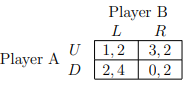
\includegraphics[scale=0.7]{./Images/Figure1.1} \\
	Figure 1.1
\end{center}
\begin{center}
	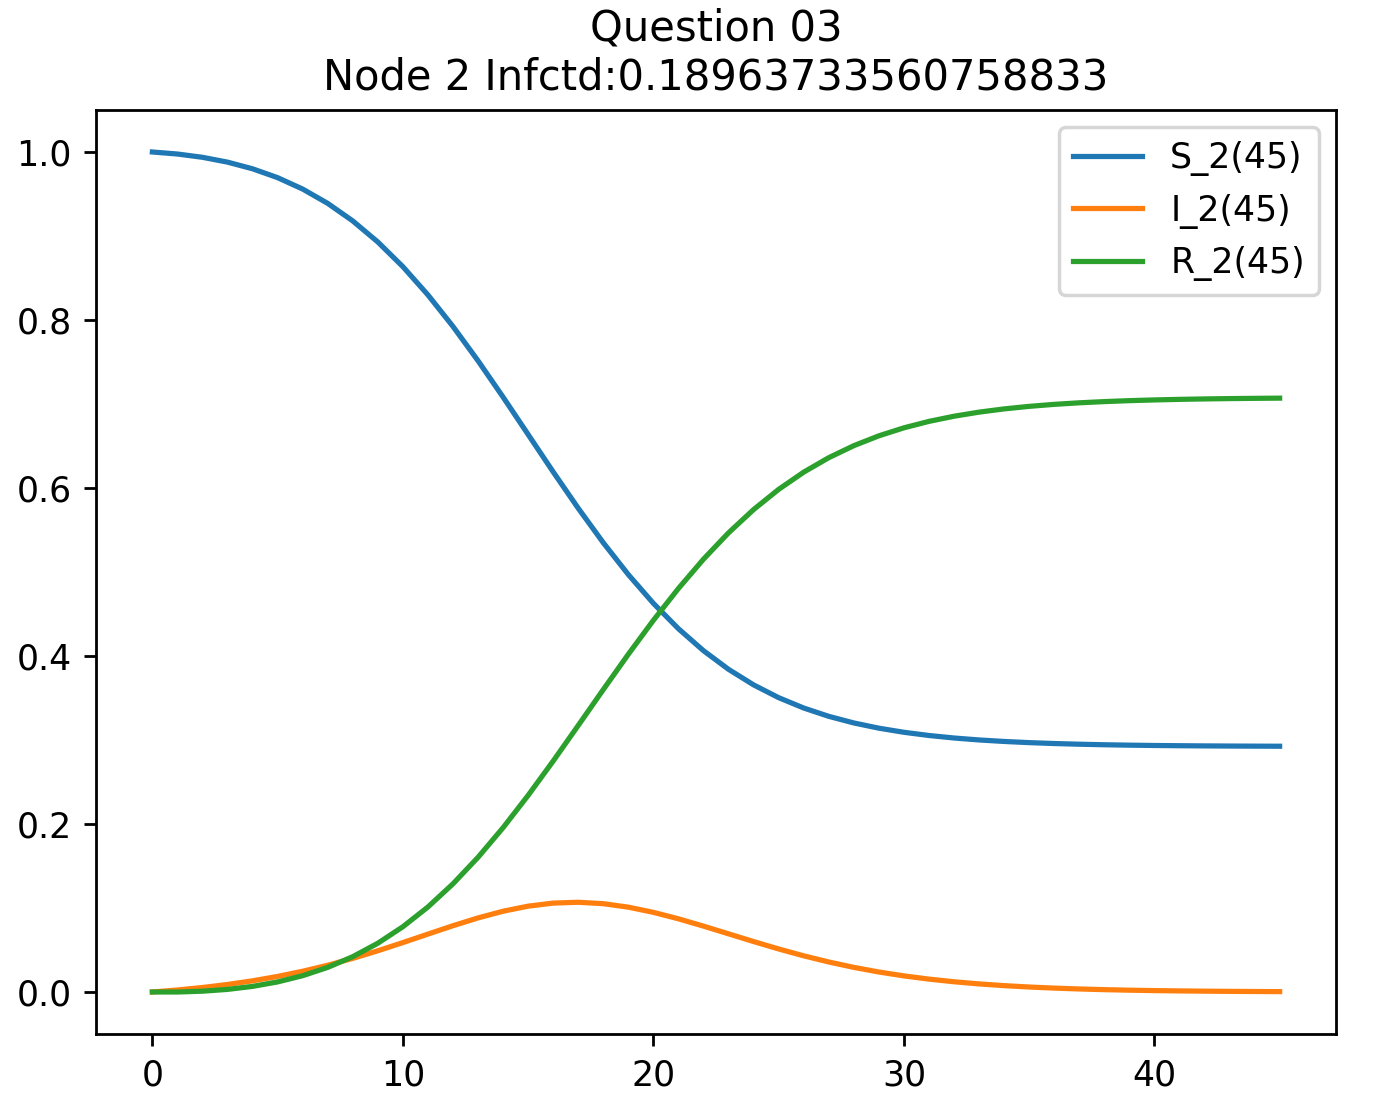
\includegraphics[scale=0.7]{./Images/Figure1.2} \\
	 Figure 1.2
\end{center}

\noindent Consider the following model of misinformation: let $x(0) = (0,\ 0, \ . \ . \ . \ , \ 0)^T$ so that everybody starts out at 0. Then, choose a node to influence (let’s say our influencing node $i$), and connect i to a new “fake” node whose initial “opinion” is 1. To make this connect, cut the weights of each of $i$’s out-edges in half, and give the new edge a weight of $0.5$. So the math works, the new fake node should have a single self-loop with weight $1$. See Figures 1.1 and 1.2 to show an example of a edge being added to node 9 to the new "fake node".  Because everybody starts out at 0, you can measure the effect of your misinformation simply by adding up everybody’s opinion. We’ll call this sum the propaganda value of your misinformation scheme, and denote it by $P(t) := \sum^{n-1}_{i=0} x_i(t)$ . An ineffective misinformation scheme would have $P(t)$ close to 0 for all time, but a very effective one would have $P(t)$ close to $n$.

% ----------------------------------------------- Implementation
\section{Implementation}  

Well to implement this first an object oriented approach was taken which was causing more over head and dependencies so a Jupyter Notebook was create to create the basic foundations for simpler to read and read code.  The following is a description of this implemented code.  First an adjacency matrix was built and hard codded into a python two dimensional array.  This we then proceed to use other code provided and earlier handout for the class to print the network out and to show that the network it represented correctly by the adjacency matrix.  
\begin{center}
	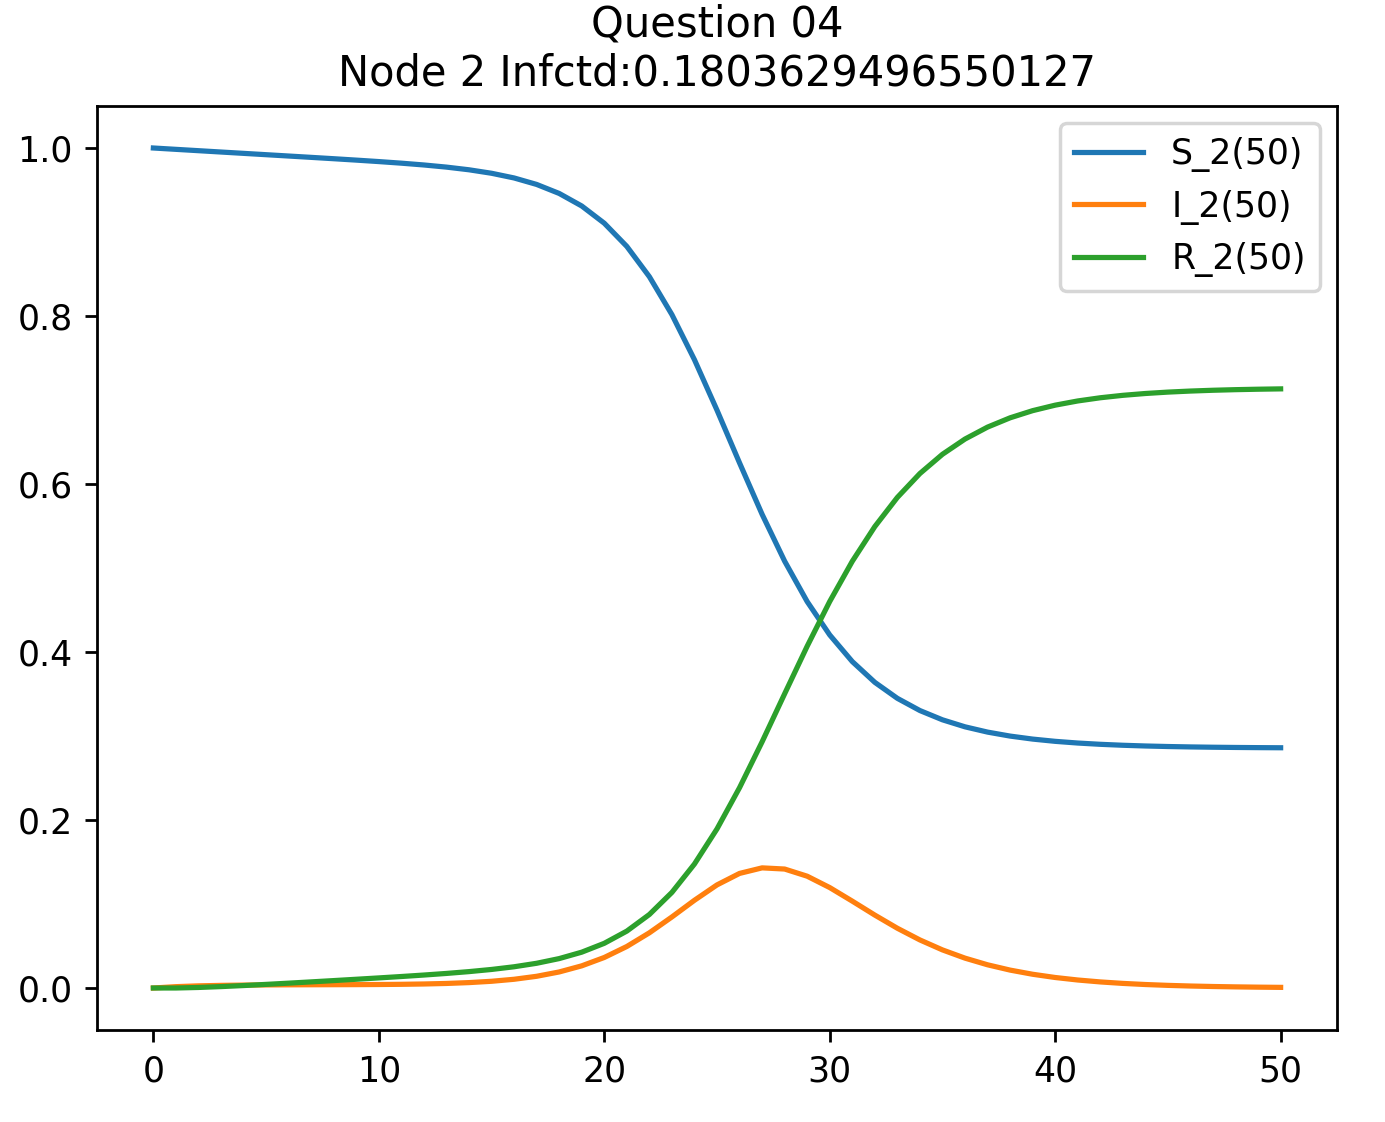
\includegraphics[scale=1.5]{./Images/Figure1.3} \\
	Figure 1.3
\end{center}
Although it might be hard to see the graph shown by Networkx that is used in a function provided to use, we can see that all the same nodes exist with the same existing edges as on the picture of the graph shown in Figure 1.1.  Now to demonstrate that we can add nodes to this adjacency matrix we build two more function that handle building the matrix and then will print it you to show that it works in connected a fake node to node 9 as in Figure 1.2.\\\\
The first function built I called addNodeToNetwork() which took two parameters which are the network we built an adjacency matrix for and the original opinions of all the existing nodes at time step $t=0$.  This functions take the network, as a two dimensional list and builds new rows with 0's added to the end of them and setting them to a new two dimension list to continue to modify before returning.  Next the two dimensional list will have a row of all zeros added at the bottom of the list. finally before returning the new network with an added node we set the new node to have a self loop and we also add a new opinion to the list or original opinions to represent the opinion of the new node which we will call the "fake node".  We also add another value to the lambda values which can be any number since it does not listen to any other nodes. The list of opinions, lambda values, and new network are then passed back. \\\\
Then the addBadEdgeToNetwork() method was created to be called right after adding a new node.  This function simply accepts three parameters to adjust the original network to having a edge between the fake node and what ever node is based as the 'node' argument.  To do this, the function multiplies every existing edge by 0.5 and then sets each element do that amount specific to the column in that node's row of edges.  Then a new edge of 0.5 is added between the fake node and the specified node.  This newly adjust network is then passed back.\\\\
After using the draw\_from\_matrix() function provided to us we can show that the matrix does in fact add a new edge.  We also checked the matrix was right by checking the console output of printing the matrix. \\
\begin{center}
	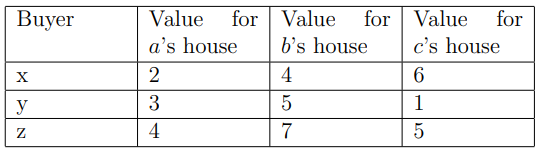
\includegraphics[scale=0.6]{./Images/Figure1.4} \\
	Figure 1.4
\end{center}
As we can see a new node has been added and the only added edge are the self loop to itslef and the new edge between node 9 and node 10, the fake node.\\\\
After verifying that this was working we used the friedkin\_johnsen() provided to us through class handouts and modified it to print out a little bit more verbose information when setting its keyword argument, show\_plot, is set to true.  This function does what has already been discussed in class by essentially using the equation as described in the introduction.  By preforming these different time steps of Friedkin-Johnsen model we were able to map the rate at which the information, or "opinion", of the "fake" spreads depending on the node that it is connected to. To perform each instance of when a different node could be connected to the "fake" node we make an abstract layer to call of the methods previously discussed so that this method or model can be called upon in a for loop of each possible neighbor that the fake node could have a connection from.  Within this model a fresh new network of the original network is made sure to be passed in to this model to represent the only connection between the fake node and any other pre-existing node.\\
Along with executing every possible connection, a list was made to capture the overall propaganda value of the network at each time step.  Another function was written to show this value as well as the opinion of each node at each iterated time step through the model and were used to display the results through other implemented methods plotAllProagandaValOverTime() \& plotAllProagandaValOverTime() to plot them individually between simulation runs and to call at the end of the for loop of all possible simulation runs to map all possible outcomes of $P(t)$ values specific to the node that the fake node was being connected from.  Unit test were also written to make sure that basic functionality is maintained through out the completion and development of this project.

% ----------------------- Execution 
\subsection{Execution}
To help mitigate any dependencies that may cause issues with running the program a requirments.txt file was provided which can be used with the below command to make sure that all the libraries used for this project are pre installed.\\
\begin{center}
py -m pip install -r requirments.txt\\
\quad \\
\end{center}
Execution is set up to simply run the missinformationProjecy.py file with the commad\\
\begin{center}
py project03.py\\
\quad \\
\end{center}
from the same working directory as this file. When running this file, without modifying it, it should save different graphs and tables to different folders within the included .zip file structure.  If the user wishes to run the file without the print out of all the graphs as they run it they must go through and uncomment out the show() method with in the functions timestepsToPTable() and plotAllProagandaValOverTime().  This will still display the tables required of in both deliverables and will be turned in from previous runs along with capbability to execute and generate "new" tables.  The overall console output has also been saved to the out tableOutput within the Outputs folder.  If there any any other questions on the over head of the project executeable refer to the README.md for futher details and help.\\

% ----------------------- Analyisis 
\subsection{Analyisis}
After personal execution with collected data and observations, I was then able to continue with providing the deliverables for the project.  First off, here is a quick overview of each deliverable asked of for this project and what it consists of.\\\\
\begin{enumerate}
	\item Implement the Friedkin-Johnsen model on the given graph. 
	\begin{enumerate}
		\setcounter{enumi}{1}
		\item  Deliverable 1: Either the computer code for your implementation, or a complete description of the maths you used to prove the other deliverables. 
	\end{enumerate}
	\item If you want to influence opinions over the short-term, which node should you influence?
	\begin{enumerate}
		\setcounter{enumi}{2}
		\item  Deliverable 2: The graph has 10 nodes; create a table which shows $P(1)$ (the total opinion of society after 1 time step) for each node to be influenced. That is, compute $P(1)$ in the case that you influence node 0; then compute $P(1)$ in the case that you influence node 1, and so on. If you care most about $P(1)$ (society’s opinions in the very short term), which node is best to influence? Which is worst? Write a few sentences explaining why you think this is the case.
	\end{enumerate}
	\item If you want to influence opinions over the long-term, which node should you influence?	
	\begin{enumerate}
		\setcounter{enumi}{3}
		\item Deliverable 3: The graph has 10 nodes; create a table which shows $P^\infty := \lim_{t to \infty} \ P(t)$ (the opinion that society converges to after a long time) for each node to be influenced. That is, compute $P^\infty$ in the case that you influence node 0; then compute $P^\infty$ in the case that you influence node 1, and so on. If you care most about $P^\infty$ (society’s opinions in the very long term), which node is best to influence? Which is worst? Write a few sentences explaining why you think this is the case. If the answer is different from what you got in Deliverable 2, try to explain why.\\\\
	\end{enumerate}
\end{enumerate}

% ----------------------- Delveriable 1 
\subsection{ Deliverable 1 }
The code for this assignment will be turned in via a .pdf file of the code that is included a .zip file with the .pdf inside the Deliverable1 folder of the .zip.  There is also output that can be generated from running the code within the unzipped project .zip folder.  The code and the .zip will take care of Deliverable 1 as well as setting up the basic file structure required for running the program within the parent directory of the unzipped folder.  For trouble shooting, a README.md is included with helpful information. 

% ----------------------- Delveriable 2
\subsection{ Deliverable 2 }
For Deliverable 2 we are to evaluate the overall networks opinions in the short term at running one time step.  Starting from time step 0, we can see see from Figure 1.5 a graph with the $P(t)$ values for each possible connection that can be made.  
\begin{center}
	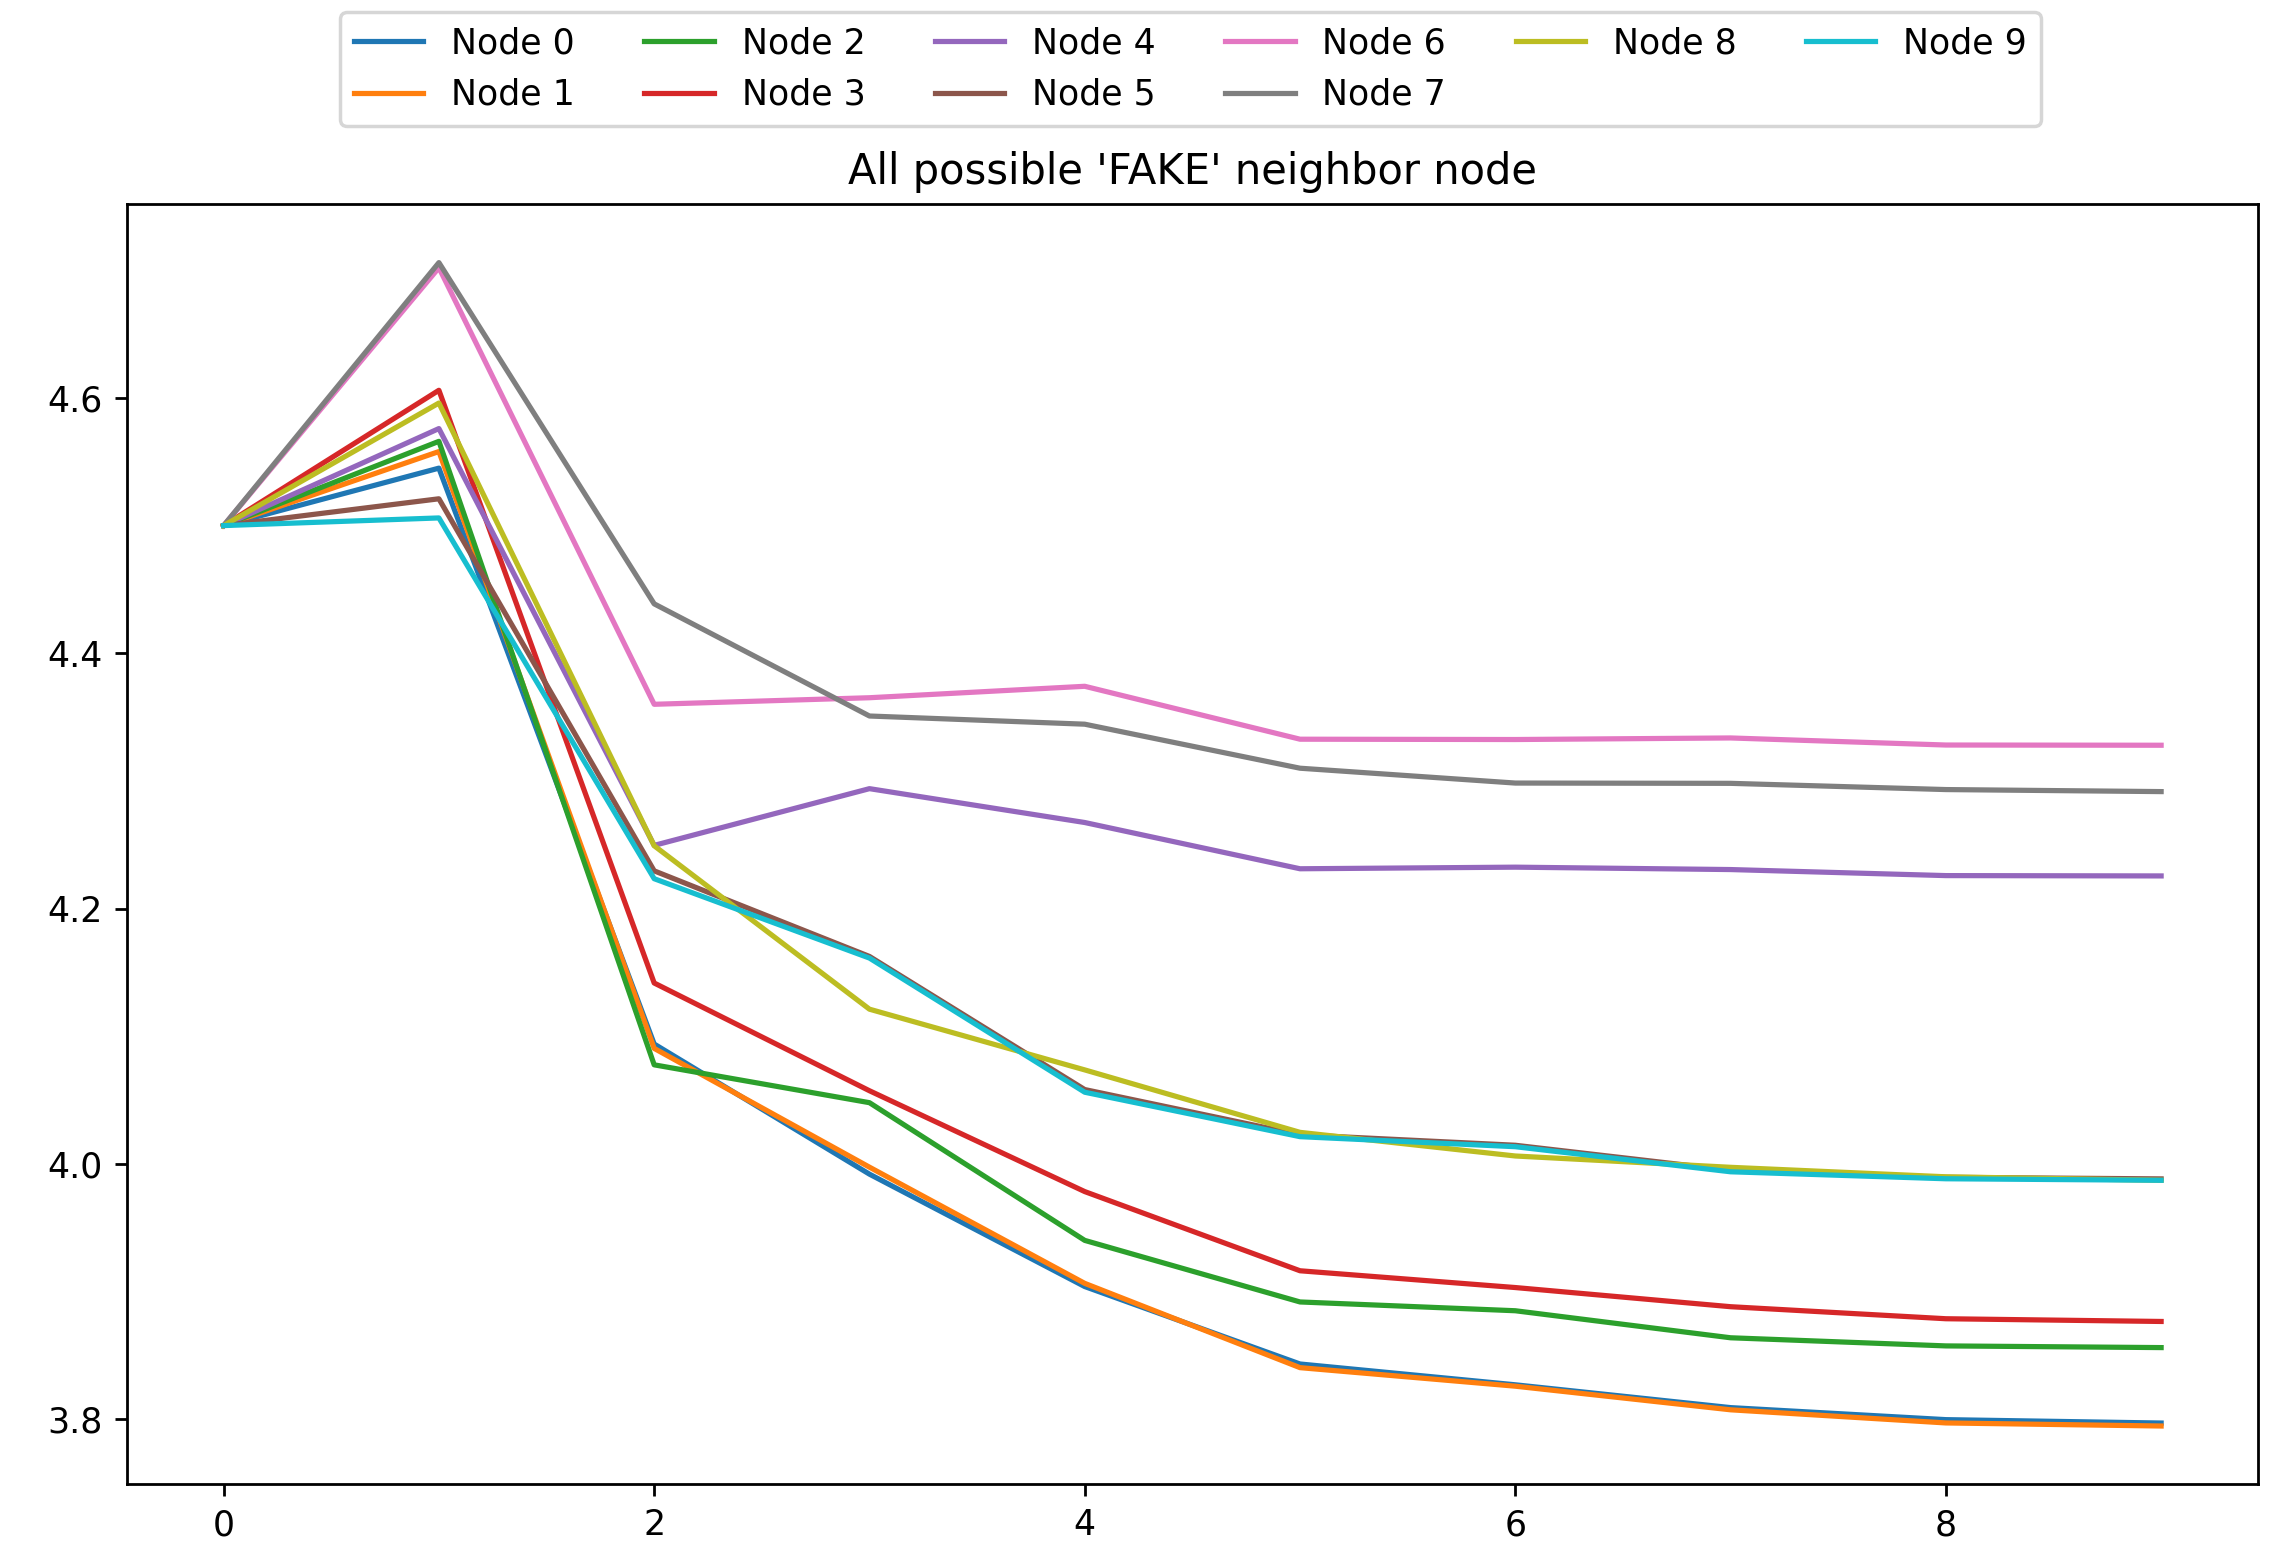
\includegraphics[scale=0.9]{./Images/Figure1.5} \\
	Figure 1.5
\end{center}
The propaganda value is plotted over 1 time step.  When lookin at this graph we see that when the fake node is being directly pointed to by nodes  9, 8, and 7, the propaganda values seem to rise to the highest.  Lets Node 9 being the highest.  Looking at the table in Figure 1.6 we can also see that there values do seem to be the highest.   As we can see having a connection from the fake node to node 9 seem to have the highest influence on the network over the first time step.  We see it gets as high as 0.475 followed by P-values of fake connections from node 8 and 7 with values 0.45 and 0.4 respectively.  This is probably due to the fact that the susceptibility of node 9 has the highest  corresponding lambda value, 0.95.  This seem to correlate with the other higher influential connections as 8 and 7 have lambda values 0.9 and 0.8. \\
\begin{center}
	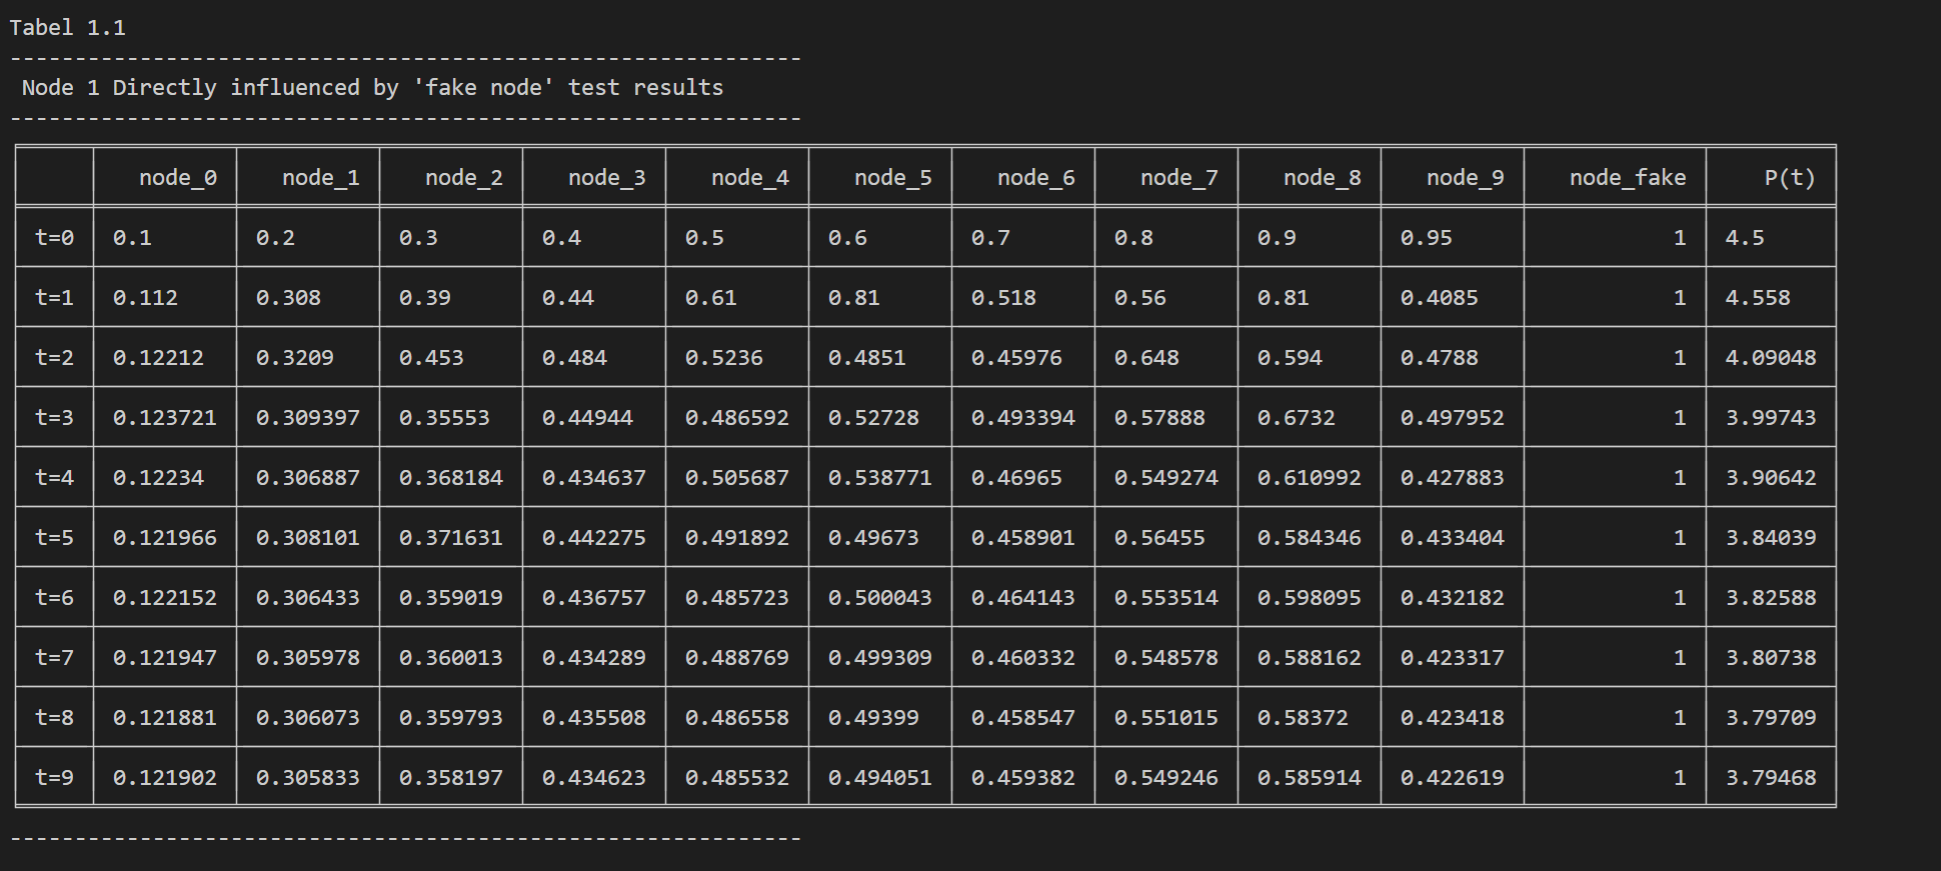
\includegraphics[scale=0.7]{./Images/Figure1.6} \\
	Figure 1.6
\end{center}
Referring back to Figure 1.4, we see that the lowest propaganda values when the connection to the fake node are the lowest at values 0, 1, and 2.  0 being the lowest at a value 0.05, followed by nodes 1 and 2 with overall $P(t)$ values 0.1 and 0.15 respectively.  We retrieved from a table generated like the one in Figure 1.6.  This also tracks with our logic since these nodes have corresponding very low lambda values.\\\\
So, we can say that if the fake node wants the influence the network the most then it should have node 9 listen to it since it is the most susceptible.  Node 0 being the lest influential node that the fake node would have little influence and low propaganda values.\\\\

% ----------------------- Delveriable 3
\subsection{ Deliverable 3}
For Deliverable 3 we are to evaluate the overall networks opinions in the long term. By looking at a graph over a longer period of time we see that the $P(t)$ values seem ton converge failry quick and flatten out over just about 10-15 time steps.  With the graph generated in Figure 1.7 we see that the $P(t)$ seem to have different correlation to the first time steps.
\begin{center}
	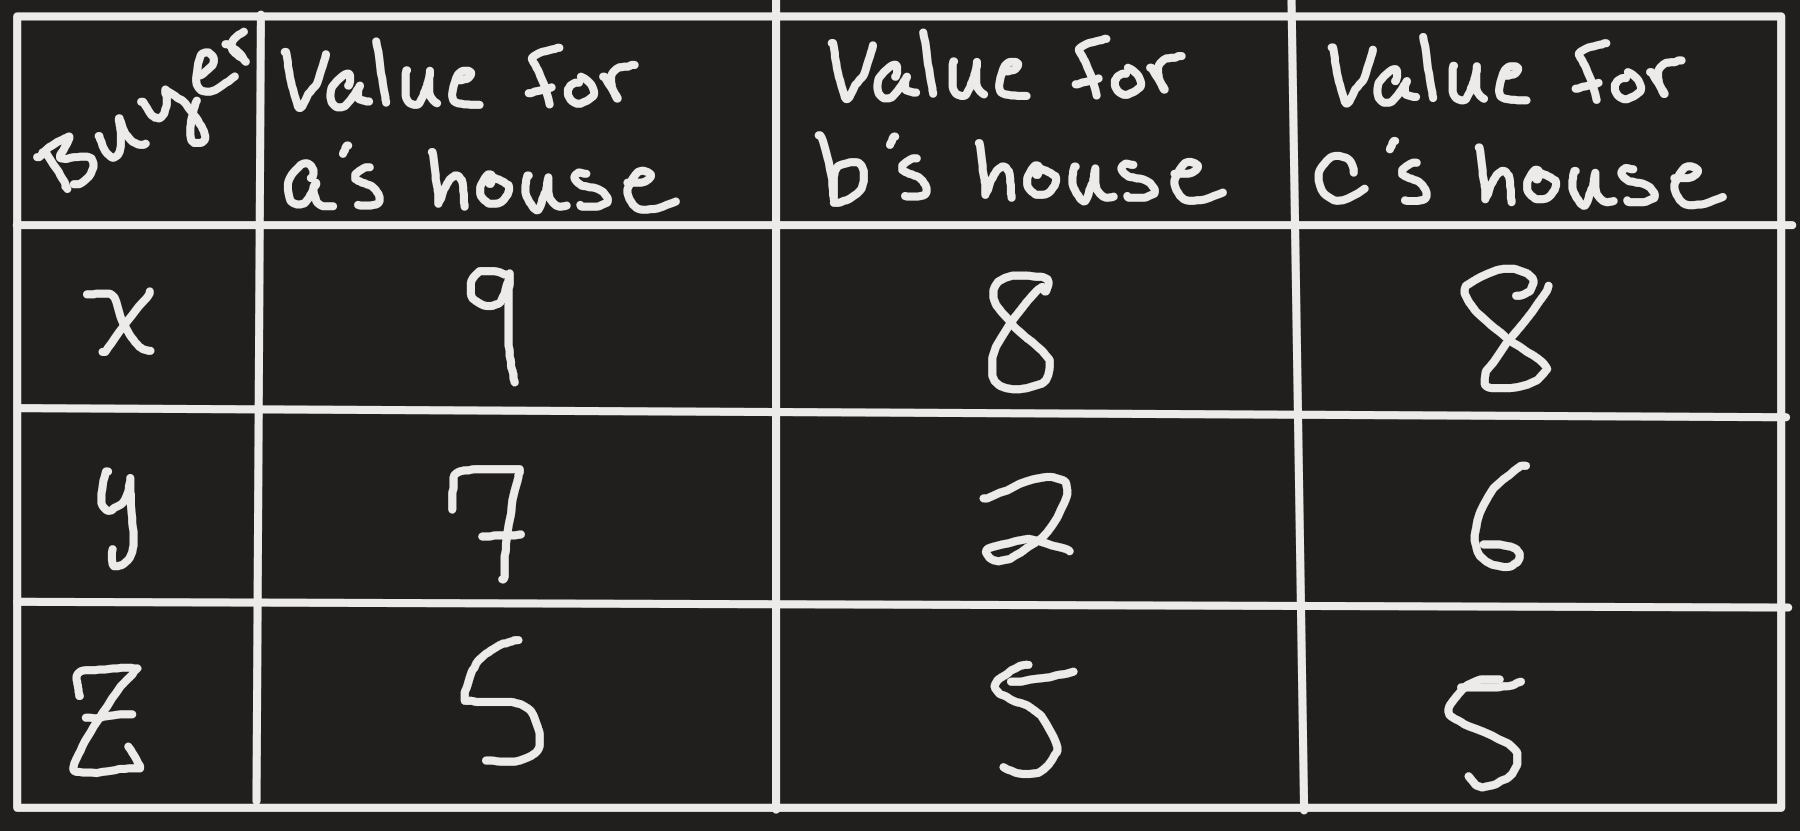
\includegraphics[scale=0.9]{./Images/Figure1.7} \\
	Figure 1.7
\end{center}
Here we can see that after just the first 10 time steps we start to see convergence of most of the nodes in just the first 3-4 time steps.  The other values do start to converge but some do have intersection points where the $P(t)$ continued to grow in the network compared to ones that were more rapidly flattening out.  For example, even though node 9 seem to have the most influential connection in the first few time steps, nodes 6 and 4 end up having a higher influence on the network than 9.  However the node with the most influence over 10 time steps was node 7, in just ten time steps the value rises from 0 to just below 1.2. Looking at the generate table shown in figure 1.8 we see that node 7 gets up to 1.4897 and does not get any higher than that.
\begin{center}
	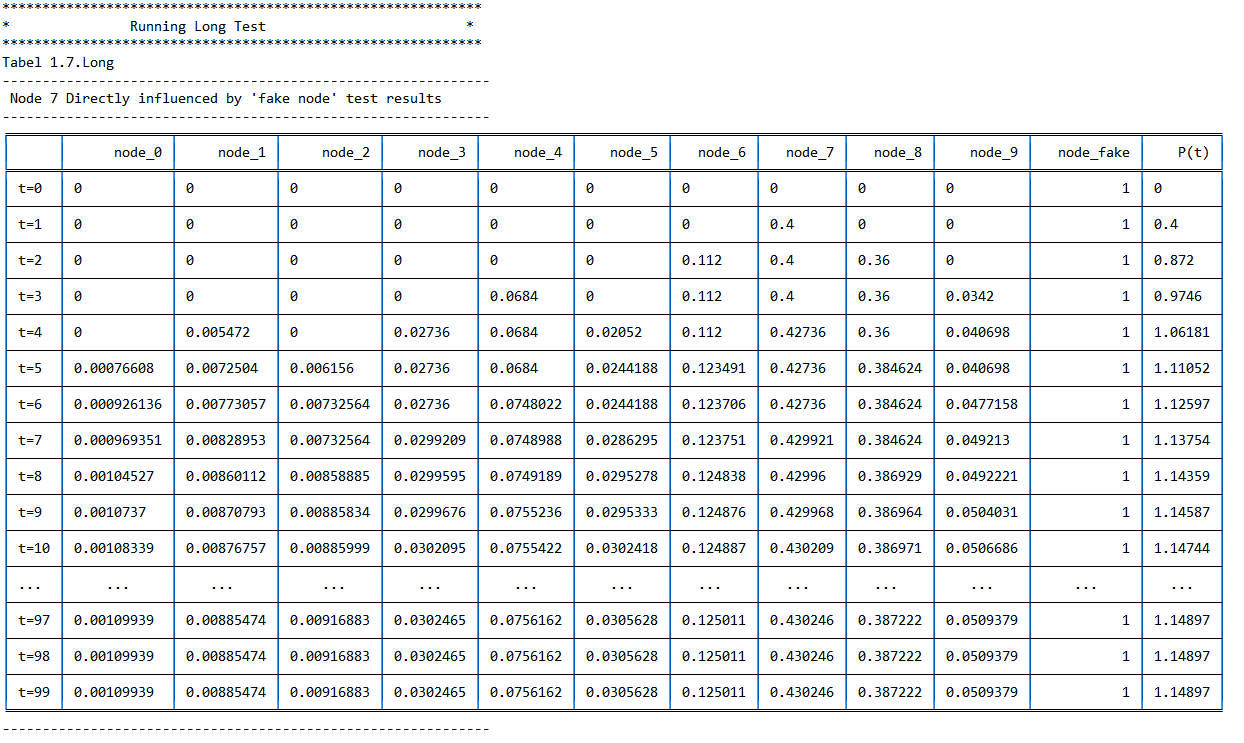
\includegraphics[scale=0.6]{./Images/Figure1.8} \\
	Figure 1.8
\end{center}
We can probably contribute this to the fact that while node 7 does have a relatively average lambda value and has two nodes listening to it. Both these nodes listening to node 7 have  high lambda values meaning higher susceptibility.  Node 8 has a 0.9 value and node 7 has a 0.8 lambda value. Node 8 has a very strong connection of 1 and node 6 has a 0.4 weight connection to 7.  These two nodes also share a connection with node 4 where node 4 has many other highly susceptible values as well.  We can also see loops with in the strongly susceptible nodes.  For the lower influential nodes, when the fake node has a connection from node 0, it continues to have the lowest influence on the network and this probably attributes to it low susceptibility as well as the fact that the only node listening to node 1 is node 0 with a even lower susceptibility.  So, in the longer runs we can see that node 7 has the highest influence on the network while node 1 seem to continue to have the lowest influence on the network.

% ----------------------------------------------- Conclusion
\section{Conclusion}

In conclusion we saw how different connection on a newtork with a node with a opnion in contrast to nodes that have none, there are many different ways and rates that the opnion can be spread through the network. When looking as very longer iteration run there were also these weird clefts that would appear a little latter after it seems like that flattening out.  In figure 1.9 we see an example where the P value seem to flatten out and then spike up a little bit real quick and flatten out again.  
\begin{center}
	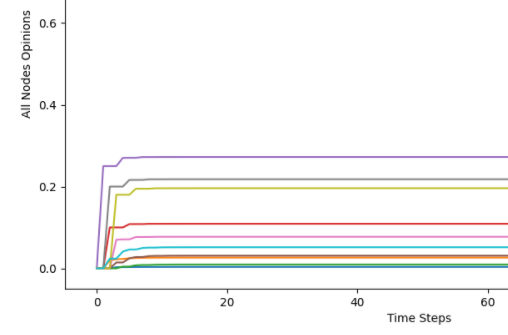
\includegraphics[scale=1.3]{./Images/Figure1.9} \\
	Figure 1.9
\end{center}
While i can't be sure what causes this exactly I have my suspensions there could be possible loops where the opnion can grow quickly when lopping through and back to a highly susceptible node. 

% ----------------------------------------------- References 
\section{References}
Credit to Dr. Philliph Brown's Jupyter note books and other class handouts, lecture and notes.\\\\
\quad\\
Networks, Crowds, and Markets: A Book by David Easley and Jon Kleinberg, https://www.cs.cornell.edu/home/kleinber/networks-book/. 

\end{document}